\documentclass[aspectratio=169,10pt]{beamer}

% -------------------------------------------------------------
% Packages & Configuration
% -------------------------------------------------------------
\usepackage[utf8]{inputenc}
\usepackage{tikz}
\usetikzlibrary{calc,positioning,shapes.geometric,arrows.meta,fit}
\usepackage{helvet}
\renewcommand{\familydefault}{\sfdefault}
\usepackage{booktabs}
\usepackage{amsmath,amssymb}
\usepackage{graphicx}
\usepackage{tcolorbox}
\usepackage{multimedia}
\usepackage{hyperref}

% Graphicspath
\graphicspath{{../Images/}{../Images/CleanPlots/}{../Images/WSS_SENSOR_OPEN/}{../Images/BRAKE_SWITCH_STUCK/}{../Images/CUTOFF_ABS_NODE/}{../}{./}}

% Remove default navigation symbols & set crisp widescreen margins
\setbeamertemplate{navigation symbols}{}
\setbeamersize{text margin left=0.55cm,text margin right=0.55cm}

% -------------------------------------------------------------
% Color Palette (Vector / Tata Automotive Theme)
% -------------------------------------------------------------
\definecolor{vectorred}{RGB}{166, 0, 44}       % Vector Corporate Crimson
\definecolor{slatedark}{RGB}{33, 37, 41}       % High-contrast charcoal
\definecolor{slategrey}{RGB}{100, 110, 120}    % Subtitle & border grey
\definecolor{cardbg}{RGB}{248, 250, 252}       % Card soft background
\definecolor{cardborder}{RGB}{212, 220, 230}   % Card border
\definecolor{accentblue}{RGB}{24, 90, 157}     % CAN Network Blue
\definecolor{accentgreen}{RGB}{22, 128, 60}    % RCA Success Green
\definecolor{accentpurple}{RGB}{112, 48, 160}  % Diagnostics Purple
\definecolor{accentamber}{RGB}{217, 119, 6}    % Fault Injection Amber

% Node & Message Colors
\definecolor{nodetester}{RGB}{112, 48, 160}     % DIAG_TESTER Diagnostics Purple
\definecolor{nodeabs}{RGB}{80, 86, 92}         % ABS/ESP Charcoal Grey
\definecolor{nodeecm}{RGB}{224, 228, 233}      % ECM Light Slate Grey
\definecolor{nodeecmtext}{RGB}{65, 72, 78}     % ECM Text Dark
\definecolor{nodetcm}{RGB}{166, 0, 44}         % TCM / Gearbox Crimson Red
\definecolor{nodebcm}{RGB}{52, 104, 152}       % BCM Slate Blue
\definecolor{busline}{RGB}{120, 128, 136}      % CAN Bus Line Grey

% Standard card tcolorbox style
\tcbset{
  cardstyle/.style={
    colback=cardbg,
    colframe=cardborder,
    boxrule=0.9pt,
    arc=5pt,
    left=6pt,right=6pt,top=4pt,bottom=4pt,
    boxsep=1pt,
    toptitle=3.5pt,bottomtitle=3.5pt,
    titlerule=0.5pt
  },
  whitecard/.style={
    colback=white,
    colframe=cardborder,
    boxrule=0.9pt,
    arc=5pt,
    left=6pt,right=6pt,top=4pt,bottom=4pt,
    boxsep=1pt,
    toptitle=3.5pt,bottomtitle=3.5pt,
    titlerule=0.5pt
  }
}

% Header & Footline Styling
\setbeamertemplate{headline}{}
\setbeamertemplate{footline}{
  \leavevmode%
  \hbox{%
    \begin{beamercolorbox}[wd=0.45\paperwidth,ht=2.4ex,dp=1.0ex,leftskip=0.55cm]{author in head/foot}%
      \tiny\color{slategrey}\textbf{Automated Root Cause Isolation in Multi-ECU Networks}
    \end{beamercolorbox}%
    \begin{beamercolorbox}[wd=0.35\paperwidth,ht=2.4ex,dp=1.0ex,center]{title in head/foot}%
      \tiny\color{slategrey}Tata Technologies TechPulse \textbar{} IVN Capstone
    \end{beamercolorbox}%
    \begin{beamercolorbox}[wd=0.20\paperwidth,ht=2.4ex,dp=1.0ex,rightskip=0.55cm,right]{date in head/foot}%
      \tiny\color{slategrey}\insertframenumber{} / \inserttotalframenumber
    \end{beamercolorbox}%
  }%
  \vskip0pt%
}

% Slide title helper
\newcommand{\slidetitle}[2]{%
  \vspace{-0.24cm}
  {\Large\bfseries\color{vectorred}#1}\\[1pt]
  {\footnotesize\color{slategrey}#2}
  \vspace{0.12cm}
}

% Custom TikZ Macros for Slide 4 Message Banners (Matching slide_3.png crisp style)
\newcommand{\msgRight}[8]{
  \begin{scope}[shift={(#1,#2)}]
    \draw[line width=1.1pt, fill=white, draw=black] (0, -0.24) rectangle (1.18, 0.24);
    \node[font=\bfseries\scriptsize, text=black, inner sep=0pt] at (0.59, 0) {#3};
    \draw[line width=1.1pt, fill=#6, draw=black] (1.18, -0.24) rectangle ({1.18+#5}, 0.24);
    \node[font=\bfseries\scriptsize, text=#7, inner sep=0pt] at ({1.18 + #5/2}, 0) {#4};
    \draw[line width=1.1pt, fill=#8, draw=black] ({1.18+#5}, -0.24) -- ({1.18+#5+0.42}, 0) -- ({1.18+#5}, 0.24) -- cycle;
  \end{scope}
}

\newcommand{\msgLeft}[8]{
  \begin{scope}[shift={(#1,#2)}]
    \draw[line width=1.1pt, fill=#8, draw=black] (0, 0) -- (0.42, -0.24) -- (0.42, 0.24) -- cycle;
    \draw[line width=1.1pt, fill=#6, draw=black] (0.42, -0.24) rectangle ({0.42+#5}, 0.24);
    \node[font=\bfseries\scriptsize, text=#7, inner sep=0pt] at ({0.42 + #5/2}, 0) {#4};
    \draw[line width=1.1pt, fill=white, draw=black] ({0.42+#5}, -0.24) rectangle ({0.42+#5+1.18}, 0.24);
    \node[font=\bfseries\scriptsize, text=black, inner sep=0pt] at ({0.42+#5+0.59}, 0) {#3};
  \end{scope}
}

\begin{document}

% =============================================================================
% SLIDE 1: Project Title and Student Details
% =============================================================================
\begin{frame}[t]
\vspace{-0.10cm}
\centering

\begin{tcolorbox}[colback=vectorred!10, colframe=vectorred!25, boxrule=0.5pt, arc=4pt, width=10.6cm, left=8pt, right=8pt, top=2.5pt, bottom=2.5pt]
  \centering\scriptsize\bfseries\color{vectorred} IN-VEHICLE NETWORKING (IVN) CAPSTONE PROJECT \quad\textbullet\quad B.TECH SEMESTER 7
\end{tcolorbox}

\vspace{0.20cm}
\resizebox{0.96\textwidth}{!}{\LARGE\bfseries\color{vectorred} Automated Root Cause Isolation in Multi-ECU Networks}\\[6pt]
{\large\bfseries\color{slatedark} Signal Dependency Mapping \& UDS Diagnostics in Vector CANoe 19}\\[5pt]
{\small\color{slategrey} Compliant with ISO 14229-1 (UDS) \textbullet{} ISO 15765-2 (DoCAN) \textbullet{} ISO 26262 ASIL-D \textbullet{} ISO 11898-1}

\vspace{0.28cm}

\begin{tcolorbox}[
  colback=cardbg, colframe=vectorred!70, boxrule=1.0pt, arc=7pt,
  width=11.4cm, left=14pt, right=14pt, top=6pt, bottom=6pt,
  colbacktitle=vectorred, coltitle=white,
  toptitle=3pt, bottomtitle=3pt,
  title={\centering\scriptsize\bfseries STUDENT DETAILS}
]
  \small\color{slatedark}
  \begin{tabular}{@{}ll@{}}
    \textbf{Name:}        & Harish R \\[2pt]
    \textbf{Roll Number:} & CB.EN.U4EEE23112 \\[2pt]
    \textbf{Degree:}      & Bachelor of Technology (B.Tech) \\[2pt]
    \textbf{Department:}  & Department of Electrical \& Electronics Engineering \\[2pt]
    \textbf{Institution:} & Amrita School of Engineering, Coimbatore \\[2pt]
    \textbf{University:}  & Amrita Vishwa Vidyapeetham
  \end{tabular}
\end{tcolorbox}

\vspace{0.20cm}
{\footnotesize\color{slategrey}\textbf{Industry Collaboration:} Tata Technologies (TechPulse Program) \quad\textbullet\quad \textbf{Platform:} Vector CANoe 19}

\end{frame}

% =============================================================================
% SLIDE 2: Problem Statement and Objectives
% =============================================================================
\begin{frame}[t]
\slidetitle{Problem Statement \& Research Objectives}{Multi-ECU Signal Cascades \textbullet{} False DTC Floods \textbullet{} ISO 26262 ASIL-D Determinism}

\begin{columns}[T,totalwidth=\textwidth]

  \begin{column}{0.485\textwidth}
    \begin{tcolorbox}[cardstyle, colframe=vectorred!75, colbacktitle=vectorred!8, height=5.55cm,
      title={\normalsize\bfseries\color{vectorred} The Problem: Cascading Alarm Floods}]
      \footnotesize\color{slatedark}\raggedright
      \begin{itemize}\setlength{\itemsep}{2.5pt}\setlength{\leftmargini}{10pt}
        \item \textbf{Dense Coupling:} Modern vehicles host 70--100 ECUs exchanging thousands of cross-dependent CAN signals.
        \item \textbf{Symptom Alarm Floods:} Single sensor or ECU faults starve healthy downstream nodes, triggering dozens of secondary DTCs.
        \item \textbf{Misdiagnosis \& Cost:} Technicians replace healthy ECUs, inflating warranty costs and extending vehicle downtime.
        \item \textbf{Safety Risk:} Conflicting DTCs confuse fail-safe controllers, risking unwanted torque cuts or phantom braking.
      \end{itemize}
    \end{tcolorbox}
  \end{column}

  \begin{column}{0.485\textwidth}
    \begin{tcolorbox}[cardstyle, colframe=accentblue!75, colbacktitle=accentblue!8, height=5.55cm,
      title={\normalsize\bfseries\color{accentblue} Project Objectives \& Contributions}]
      \footnotesize\color{slatedark}\raggedright
      \begin{itemize}\setlength{\itemsep}{2.5pt}\setlength{\leftmargini}{10pt}
        \item \textbf{DAG Signal Modeling:} Formulate in-vehicle signal flows as a Directed Acyclic Graph $G=(V, E)$ capturing causal links.
        \item \textbf{On-Bus Pruning Engine:} Implement in-degree topological filtering in CAPL to isolate root causes in real time.
        \item \textbf{Deterministic Timing:} Achieve disambiguation in $<50$ ms, within the ISO 26262 ASIL-D 100 ms FTTI bound.
        \item \textbf{Vector CANoe 19 Validation:} Validate across 6 failure modes (sensor shorts, ECU dropouts, stuck switches) at 100\% accuracy.
      \end{itemize}
    \end{tcolorbox}
  \end{column}

\end{columns}

\vspace{0.12cm}
\begin{tcolorbox}[colback=slategrey!10, colframe=cardborder, boxrule=0.7pt, arc=4pt, left=6pt, right=6pt, top=3.5pt, bottom=3.5pt]
  \centering\scriptsize\color{slatedark}
  \textbf{Target Scope:} 4 Distributed ECUs (ECM, ABS, TCM, BCM) \quad\textbullet\quad 15 CAN Messages \quad\textbullet\quad 43 Powertrain \& Chassis Signals \quad\textbullet\quad 500 kbps CAN
\end{tcolorbox}

\end{frame}

% =============================================================================
% SLIDE 3: System Architecture & Block Diagram (Clean Orthogonal Layout)
% =============================================================================
\begin{frame}[t]
\slidetitle{Detailed System Architecture}{Multi-Layer Automotive E/E Simulation Architecture in Vector CANoe 19}

\centering
\vspace{-0.12cm}
\resizebox{\textwidth}{!}{%
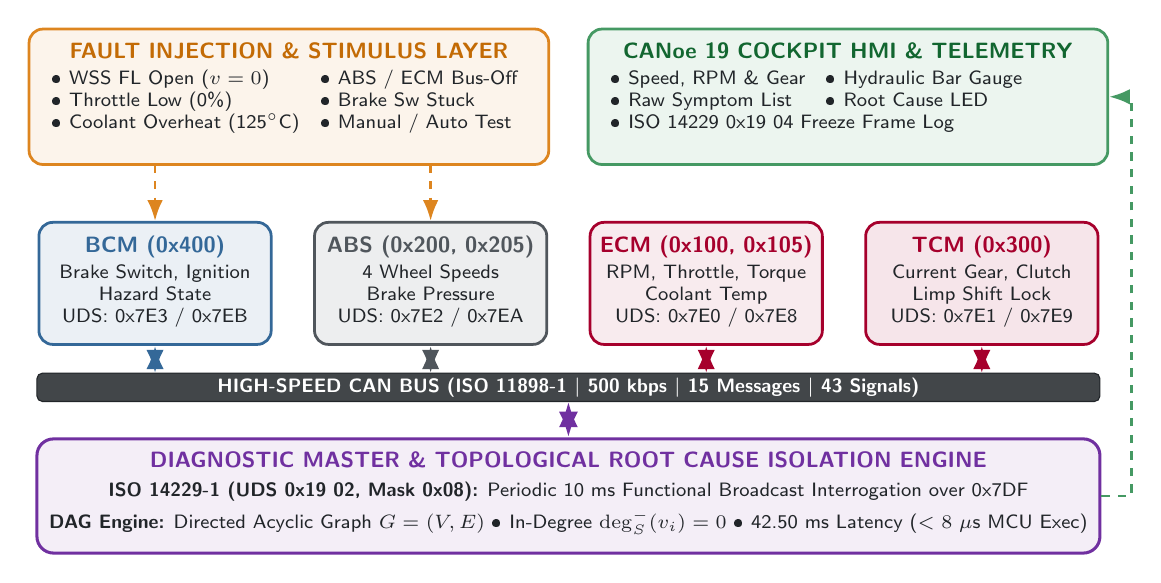
\begin{tikzpicture}[x=1cm, y=1cm, >=Latex]

  % LAYER 1 (Top): Balanced Wide Stimulus & HMI Cards
  \node[draw=accentamber!90, fill=accentamber!8, rounded corners=5pt, line width=1.0pt, minimum width=6.6cm, minimum height=1.72cm] (inj_box) at (3.45, 4.72) {};
  \node[font=\bfseries\footnotesize, text=accentamber!90!black, anchor=north] at ($(inj_box.north)+(0,-0.07)$) {FAULT INJECTION \& STIMULUS LAYER};
  \node[font=\scriptsize, text=slatedark, anchor=north west] at ($(inj_box.north west)+(0.18,-0.40)$) {
    \begin{tabular}{@{}l@{\quad}l@{}}
      \textbullet~WSS FL Open ($v=0$) & \textbullet~ABS / ECM Bus-Off \\
      \textbullet~Throttle Low (0\%)    & \textbullet~Brake Sw Stuck \\
      \textbullet~Coolant Overheat (125$^\circ$C) & \textbullet~Manual / Auto Test
    \end{tabular}
  };

  \node[draw=accentgreen!80, fill=accentgreen!8, rounded corners=5pt, line width=1.0pt, minimum width=6.6cm, minimum height=1.72cm] (hmi_box) at (10.55, 4.72) {};
  \node[font=\bfseries\footnotesize, text=accentgreen!80!black, anchor=north] at ($(hmi_box.north)+(0,-0.07)$) {CANoe 19 COCKPIT HMI \& TELEMETRY};
  \node[font=\scriptsize, text=slatedark, anchor=north west] at ($(hmi_box.north west)+(0.18,-0.40)$) {
    \begin{tabular}{@{}l@{\quad}l@{}}
      \textbullet~Speed, RPM \& Gear    & \textbullet~Hydraulic Bar Gauge \\
      \textbullet~Raw Symptom List      & \textbullet~Root Cause LED \\
      \multicolumn{2}{@{}l@{}}{\textbullet~ISO 14229 0x19 04 Freeze Frame Log}
    \end{tabular}
  };

  % LAYER 2 (Middle): 4 Evenly Spaced ECUs
  \node[draw=nodebcm, fill=nodebcm!10, rounded corners=5pt, line width=1.0pt, minimum width=2.95cm, minimum height=1.55cm] (bcm) at (1.75, 2.35) {};
  \node[font=\bfseries\footnotesize, text=nodebcm, anchor=north] at ($(bcm.north)+(0,-0.06)$) {BCM (0x400)};
  \node[font=\scriptsize, text=slatedark, align=center, anchor=center] at ($(bcm.center)+(0,-0.16)$) {Brake Switch, Ignition\\Hazard State\\UDS: 0x7E3 / 0x7EB};

  \node[draw=nodeabs, fill=nodeabs!10, rounded corners=5pt, line width=1.0pt, minimum width=2.95cm, minimum height=1.55cm] (abs) at (5.25, 2.35) {};
  \node[font=\bfseries\footnotesize, text=nodeabs, anchor=north] at ($(abs.north)+(0,-0.06)$) {ABS (0x200, 0x205)};
  \node[font=\scriptsize, text=slatedark, align=center, anchor=center] at ($(abs.center)+(0,-0.16)$) {4 Wheel Speeds\\Brake Pressure\\UDS: 0x7E2 / 0x7EA};

  \node[draw=vectorred, fill=vectorred!8, rounded corners=5pt, line width=1.0pt, minimum width=2.95cm, minimum height=1.55cm] (ecm) at (8.75, 2.35) {};
  \node[font=\bfseries\footnotesize, text=vectorred, anchor=north] at ($(ecm.north)+(0,-0.06)$) {ECM (0x100, 0x105)};
  \node[font=\scriptsize, text=slatedark, align=center, anchor=center] at ($(ecm.center)+(0,-0.16)$) {RPM, Throttle, Torque\\Coolant Temp\\UDS: 0x7E0 / 0x7E8};

  \node[draw=nodetcm, fill=nodetcm!10, rounded corners=5pt, line width=1.0pt, minimum width=2.95cm, minimum height=1.55cm] (tcm) at (12.25, 2.35) {};
  \node[font=\bfseries\footnotesize, text=nodetcm, anchor=north] at ($(tcm.north)+(0,-0.06)$) {TCM (0x300)};
  \node[font=\scriptsize, text=slatedark, align=center, anchor=center] at ($(tcm.center)+(0,-0.16)$) {Current Gear, Clutch\\Limp Shift Lock\\UDS: 0x7E1 / 0x7E9};

  % HIGH-SPEED CAN BUS BAR
  \filldraw[fill=slatedark!85, draw=slatedark, rounded corners=2pt] (0.25, 0.85) rectangle (13.75, 1.21);
  \node[font=\bfseries\scriptsize, text=white] at (7.0, 1.03) {HIGH-SPEED CAN BUS (ISO 11898-1 \textbar{} 500 kbps \textbar{} 15 Messages \textbar{} 43 Signals)};

  % ECU <-> Bus orthogonal connectors
  \draw[line width=1.2pt, <->, color=nodebcm]   (bcm.south) -- (1.75, 1.21);
  \draw[line width=1.2pt, <->, color=nodeabs]   (abs.south) -- (5.25, 1.21);
  \draw[line width=1.2pt, <->, color=vectorred] (ecm.south) -- (8.75, 1.21);
  \draw[line width=1.2pt, <->, color=nodetcm]   (tcm.south) -- (12.25, 1.21);

  % LAYER 3 (Bottom): Diagnostic Master & DAG Engine (Clean 2-line layout!)
  \node[draw=nodetester, fill=nodetester!8, rounded corners=6pt, line width=1.1pt, minimum width=13.5cm, minimum height=1.45cm] (diag_box) at (7.0, -0.35) {};
  \node[font=\bfseries\footnotesize, text=nodetester, anchor=north] at ($(diag_box.north)+(0,-0.06)$) {DIAGNOSTIC MASTER \& TOPOLOGICAL ROOT CAUSE ISOLATION ENGINE};
  \node[font=\scriptsize, text=slatedark, align=center, anchor=center] at ($(diag_box.center)+(0,-0.16)$) {
    \textbf{ISO 14229-1 (UDS 0x19 02, Mask 0x08):} Periodic 10 ms Functional Broadcast Interrogation over 0x7DF\\[2pt]
    \textbf{DAG Engine:} Directed Acyclic Graph $G=(V, E)$ \textbullet{} In-Degree $\deg_S^-(v_i) = 0$ \textbullet{} 42.50 ms Latency ($<8~\mu$s MCU Exec)
  };

  % Clean Bus <-> Master arrow
  \draw[line width=1.4pt, <->, color=nodetester] (7.0, 0.85) -- (diag_box.north);

  % Clean Non-Overlapping Inter-Layer Links
  \draw[line width=1.0pt, ->, dashed, color=accentamber!90] (1.75, 3.86) -- (bcm.north);
  \draw[line width=1.0pt, ->, dashed, color=accentamber!90] (5.25, 3.86) -- (abs.north);
  \draw[line width=1.0pt, ->, dashed, color=accentgreen!80] (diag_box.east) -- (14.15, -0.35) |- (hmi_box.east);

\end{tikzpicture}%
}

\end{frame}

% =============================================================================
% SLIDE 4: CAN Network Message and Signal Structure (Based on slide_3.png)
% =============================================================================
\begin{frame}[t]
\slidetitle{Node, Message and Signal Structure}{Vehicle E/E Architecture \textbullet{} High-Speed CAN 500 kbps (ISO 11898-1) \textbullet{} CAN Arbitration Priority Ordering}

\centering
\vspace{-0.10cm}
\resizebox{\textwidth}{!}{%
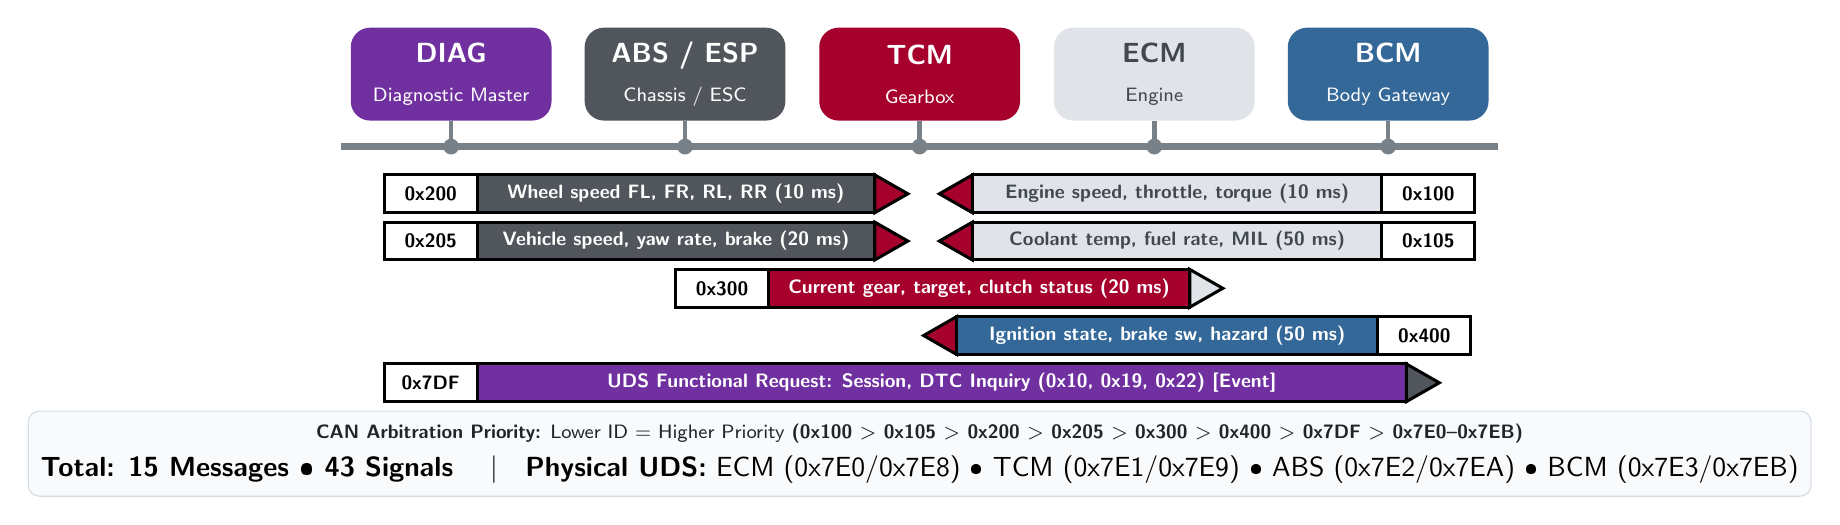
\begin{tikzpicture}[x=1cm, y=1cm]

  % 5 Nodes Across Top (Exact order & colors matching slide_3.png)
  \node[draw=none, fill=nodetester, rounded corners=7pt, minimum width=2.55cm, minimum height=1.18cm, text=white, align=center] (n_diag) at (1.45, 3.30) {\textbf{\normalsize DIAG}\\[2pt]\scriptsize Diagnostic Master};
  \node[draw=none, fill=nodeabs,    rounded corners=7pt, minimum width=2.55cm, minimum height=1.18cm, text=white, align=center] (n_abs)  at (4.42, 3.30) {\textbf{\normalsize ABS / ESP}\\[2pt]\scriptsize Chassis / ESC};
  \node[draw=none, fill=nodetcm,    rounded corners=7pt, minimum width=2.55cm, minimum height=1.18cm, text=white, align=center] (n_tcm)  at (7.40, 3.30) {\textbf{\normalsize TCM}\\[2pt]\scriptsize Gearbox};
  \node[draw=none, fill=nodeecm,    rounded corners=7pt, minimum width=2.55cm, minimum height=1.18cm, text=nodeecmtext, align=center] (n_ecm)  at (10.38, 3.30) {\textbf{\normalsize ECM}\\[2pt]\scriptsize Engine};
  \node[draw=none, fill=nodebcm,    rounded corners=7pt, minimum width=2.55cm, minimum height=1.18cm, text=white, align=center] (n_bcm)  at (13.35, 3.30) {\textbf{\normalsize BCM}\\[2pt]\scriptsize Body Gateway};

  % Bus Line & Drop Dots
  \draw[line width=2.4pt, color=busline] (0.05, 2.38) -- (14.75, 2.38);
  \foreach \x in {1.45, 4.42, 7.40, 10.38, 13.35} {
    \draw[line width=1.6pt, color=busline] (\x, 2.71) -- (\x, 2.38);
    \fill[busline] (\x, 2.38) circle (0.10);
  }

  % Message Banners (Clean vertical spacing so 0x7DF never touches footer!)
  % Row 1: 0x200 (ABS -> right) & 0x100 (left <- ECM)
  \msgRight{0.60}{1.78}{0x200}{Wheel speed FL, FR, RL, RR (10 ms)}{5.05}{nodeabs}{white}{nodetcm}
  \msgLeft {7.65}{1.78}{0x100}{Engine speed, throttle, torque (10 ms)}{5.20}{nodeecm}{nodeecmtext}{nodetcm}

  % Row 2: 0x205 (ABS -> right) & 0x105 (left <- ECM)
  \msgRight{0.60}{1.18}{0x205}{Vehicle speed, yaw rate, brake (20 ms)}{5.05}{nodeabs}{white}{nodetcm}
  \msgLeft {7.65}{1.18}{0x105}{Coolant temp, fuel rate, MIL (50 ms)}{5.20}{nodeecm}{nodeecmtext}{nodetcm}

  % Row 3: 0x300 (TCM -> right)
  \msgRight{4.30}{0.58}{0x300}{Current gear, target, clutch status (20 ms)}{5.35}{nodetcm}{white}{nodeecm}

  % Row 4: 0x400 (left <- BCM)
  \msgLeft {7.45}{-0.02}{0x400}{Ignition state, brake sw, hazard (50 ms)}{5.35}{nodebcm}{white}{nodetcm}

  % Row 5: 0x7DF (DIAG Functional Req across full bus)
  \msgRight{0.60}{-0.62}{0x7DF}{UDS Functional Request: Session, DTC Inquiry (0x10, 0x19, 0x22) [Event]}{11.80}{nodetester}{white}{nodeabs}

  % Priority Rule & Physical UDS Mapping Footer (Strictly 2 crisp lines cleanly separated!)
  \node[draw=cardborder, fill=cardbg, rounded corners=4pt, inner sep=4.5pt, minimum width=14.6cm, align=center] at (7.40, -1.52) {
    \scriptsize\color{slatedark}
    \textbf{CAN Arbitration Priority:} Lower ID = Higher Priority \textbf{(0x100 $>$ 0x105 $>$ 0x200 $>$ 0x205 $>$ 0x300 $>$ 0x400 $>$ 0x7DF $>$ 0x7E0--0x7EB)}\\[2pt]
    \textbf{Total: 15 Messages \textbullet{} 43 Signals} \quad\textbar\quad \textbf{Physical UDS:} ECM (0x7E0/0x7E8) \textbullet{} TCM (0x7E1/0x7E9) \textbullet{} ABS (0x7E2/0x7EA) \textbullet{} BCM (0x7E3/0x7EB)
  };

\end{tikzpicture}%
}

\end{frame}

% =============================================================================
% SLIDE 5: Implementation Methodology – Directed Acyclic Graph (DAG) & Pruning
% =============================================================================
\begin{frame}[t]
\slidetitle{Implementation Methodology: DAG Pruning Algorithm}{Mathematical Formulation \textbullet{} Graph Topology \textbullet{} In-Degree Evaluation Loop}

\begin{columns}[T,totalwidth=\textwidth]

  % Column 1: DAG Formulation & Math (Fits comfortably inside 6.40cm card!)
  \begin{column}{0.485\textwidth}
    \begin{tcolorbox}[cardstyle, colframe=vectorred!70, colbacktitle=vectorred!8, height=6.40cm,
      title={\normalsize\bfseries\color{vectorred} 1. Graph Formulation \& In-Degree}]
      \footnotesize\color{slatedark}\raggedright
      DAG $G = (V, E)$ models causal fault dependencies:
      \vspace{-3pt}
      \begin{itemize}\setlength{\itemsep}{1.5pt}\setlength{\leftmargini}{10pt}
        \item \textbf{Vertices:} $V=\{v_1{=}\text{ECM}, v_2{=}\text{ABS}, v_3{=}\text{TCM}, v_4{=}\text{BCM}\}$.
        \item \textbf{Edges:} $(v_i, v_j) \in E \iff v_j$ reads signals from $v_i$.
        \item \textbf{Failure Set ($S$):} Active DTC ECUs via UDS 0x19 02.
      \end{itemize}
      \vspace{-2pt}
      \vspace{2pt}
      \textbf{Restricted In-Degree Metric:}\par
      \vspace{2pt}
      {\centering$\displaystyle \deg_S^-(v_i) = \sum_{v_j \in S} A_{ji}$\par}
      \vspace{4pt}
      \textbf{Isolation Decision Rule:}\par
      \vspace{2pt}
      {\centering$\deg_S^-(v_i) = 0 \implies \text{\textbf{Root Cause Node}}$\par}
      \vspace{2pt}
      {\centering$\deg_S^-(v_i) \ge 1 \implies \text{\textbf{Suppressed Symptom DTC}}$\par}
    \end{tcolorbox}
  \end{column}

  % Column 2: Visual Topology & Algorithmic Workflow
  \begin{column}{0.485\textwidth}
    \begin{tcolorbox}[cardstyle, colframe=accentblue!70, colbacktitle=accentblue!8, height=6.40cm,
      title={\normalsize\bfseries\color{accentblue} 2. Topology \& Algorithmic Workflow}]
      \centering
      \vspace{1pt}
      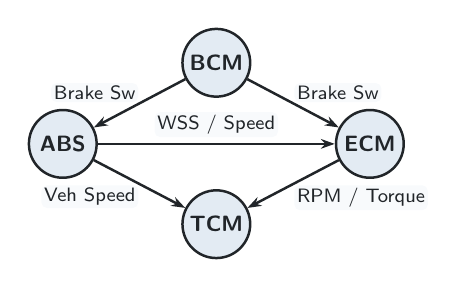
\begin{tikzpicture}[
          x=1cm, y=1cm,
          ecunode/.style={circle, draw=slatedark, fill=accentblue!12, line width=0.9pt, font=\sffamily\footnotesize\bfseries, text=slatedark, align=center, minimum size=0.86cm, inner sep=1pt},
          edgearr/.style={-{Stealth[length=5pt, width=3.5pt]}, line width=0.9pt, draw=slatedark},
          edgelabel/.style={font=\sffamily\scriptsize, fill=cardbg, inner sep=1pt, rounded corners=2pt, text=slatedark}
      ]
        \node[ecunode] (bcm) at (0, 2.05) {BCM};
        \node[ecunode] (abs) at (-1.95, 1.02) {ABS};
        \node[ecunode] (ecm) at (1.95, 1.02) {ECM};
        \node[ecunode] (tcm) at (0, 0) {TCM};

        \draw[edgearr] (bcm) -- (abs) node[edgelabel, midway, above left] {Brake Sw};
        \draw[edgearr] (bcm) -- (ecm) node[edgelabel, midway, above right] {Brake Sw};
        \draw[edgearr] (abs) -- (ecm) node[edgelabel, midway, above=2pt] {WSS / Speed};
        \draw[edgearr] (abs) -- (tcm) node[edgelabel, midway, below left] {Veh Speed};
        \draw[edgearr] (ecm) -- (tcm) node[edgelabel, midway, below right] {RPM / Torque};
      \end{tikzpicture}

      \vspace{4pt}
      \begin{minipage}{0.96\linewidth}
        \footnotesize\color{slatedark}\raggedright
        \textbf{Execution Steps:}\\[2pt]
        1. Poll all ECUs via UDS 0x19 02 (mask 0x08).\\
        2. Populate active DTC nodes into subgraph $S$.\\
        3. Compute in-degree $\deg_S^-(v)$ via matrix lookup.\\
        4. Isolate $\deg_S^-(v) = 0$ as Root Cause; prune rest.
      \end{minipage}
    \end{tcolorbox}
  \end{column}

\end{columns}

\end{frame}

% =============================================================================
% SLIDE 6: Vector CANoe 19 Simulation Setup & Diagnostic Cockpit Panel
% =============================================================================
\begin{frame}[t]
\slidetitle{Vector CANoe 19 Simulation \& Diagnostic Panel}{Virtual Vehicle Telemetry \textbullet{} Interactive Instrument Cluster \textbullet{} Real-Time CAPL Engine}

\begin{columns}[T,totalwidth=\textwidth]

  \begin{column}{0.46\textwidth}
    \begin{tcolorbox}[cardstyle, colframe=vectorred!70, colbacktitle=vectorred!8, height=6.35cm,
      title={\normalsize\bfseries\color{vectorred} Virtual Network Environment}]
      \footnotesize\color{slatedark}\raggedright
      \vspace{-2pt}
      \begin{itemize}\setlength{\itemsep}{1.5pt}\setlength{\leftmargini}{10pt}
        \item \textbf{Vector CANoe 19 Engine:} Simulates complete 500 kbps CAN bus with event-driven CAPL node logic.
        \item \textbf{Realistic Vehicle Physics:} 4-wheel speeds, engine dynamics, gear shifts, and hydraulic braking.
        \item \textbf{Interactive Fault Injection:} Toggle switches inject open circuits, sensor shorts, and node dropouts.
        \item \textbf{Automated UDS Master:} Periodic CAPL timer polls 0x7DF every 10 ms; parses 0x59 into DAG bitmasks.
        \item \textbf{Zero-Jitter Execution:} Disambiguation runs in $<8~\mu$s with zero scheduling overhead.
      \end{itemize}
    \end{tcolorbox}
  \end{column}

  \begin{column}{0.52\textwidth}
    \begin{tcolorbox}[whitecard, height=6.35cm]
      \centering
      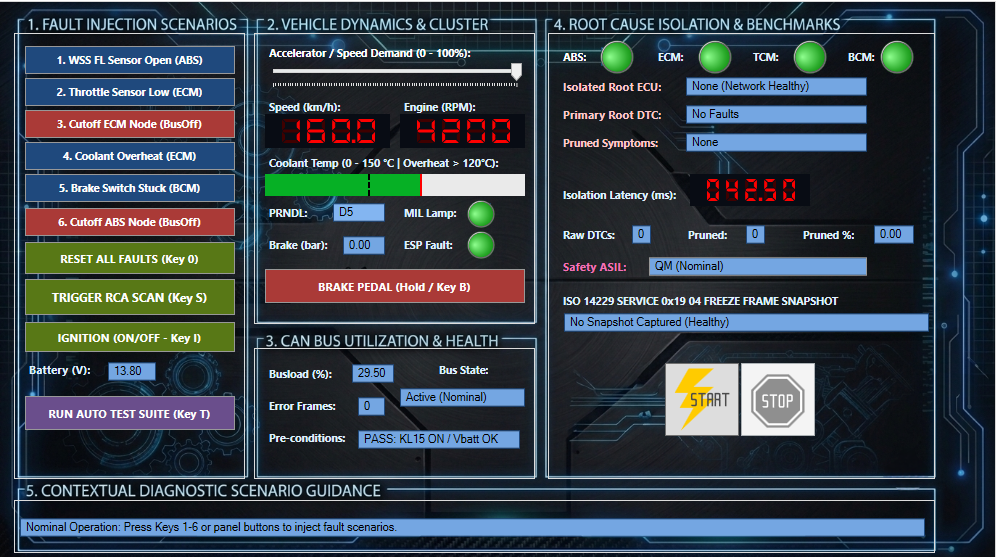
\includegraphics[width=\linewidth, height=4.65cm, keepaspectratio]{PANEL_NORMAL.png}\\[6pt]
      \footnotesize\color{slategrey}
      \textbf{CANoe 19 Cockpit HMI:} Fault-free cruise at 160.0 km/h (4200 RPM, 5th gear D5), showing healthy green status across all 4 ECUs.
    \end{tcolorbox}
  \end{column}

\end{columns}

\end{frame}

% =============================================================================
% SLIDE 7: Demonstration of Solution – Multi-Scenario Fault Isolation
% =============================================================================
\begin{frame}[t]
\slidetitle{Solution Demonstration: Multi-Scenario Fault Isolation}{6 Real-World Failure Modes \textbullet{} 100\% Disambiguation Accuracy \textbullet{} Zero False Replacements}

\begin{columns}[T,totalwidth=\textwidth]

  \begin{column}{0.485\textwidth}
    \begin{tcolorbox}[cardstyle, colframe=vectorred!70, colbacktitle=vectorred!8, height=5.25cm,
      title={\footnotesize\bfseries\color{vectorred} Scenario 1: Wheel Speed Sensor Open (ASIL-D)}]
      \centering
      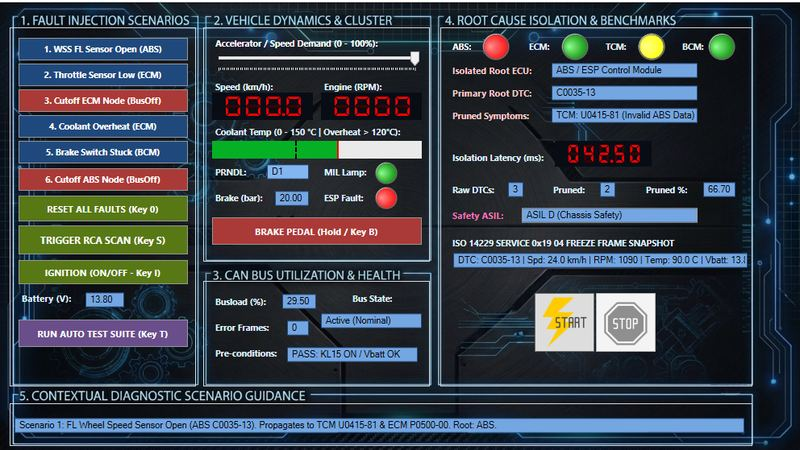
\includegraphics[width=\linewidth, height=2.65cm, keepaspectratio]{WSS_SENSOR_OPEN/PANEL.jpg}\\[4pt]
      \begin{minipage}{0.98\linewidth}
        \scriptsize\color{slatedark}\raggedright
        \textbf{Raw Codes:} ABS (C0035-13), ECM (P0500-00), TCM (U0415-81).\\[2pt]
        \textbf{Topological Result:} ABS isolated ($\deg_S^- = 0$); ECM \& TCM suppressed ($\deg_S^- \ge 1$). 66.7\% DTC reduction; TCM enters speed-gated limp mode.
      \end{minipage}
    \end{tcolorbox}
  \end{column}

  \begin{column}{0.485\textwidth}
    \begin{tcolorbox}[cardstyle, colframe=accentblue!70, colbacktitle=accentblue!8, height=5.25cm,
      title={\footnotesize\bfseries\color{accentblue} Scenario 5: Brake Switch Stuck Closed (ASIL-B)}]
      \centering
      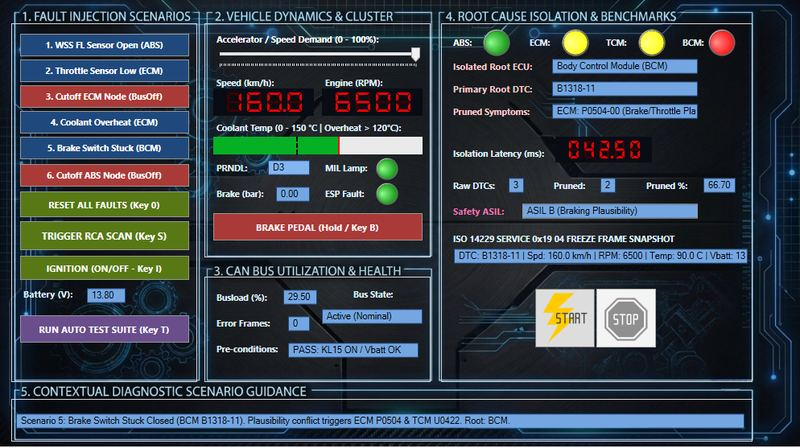
\includegraphics[width=\linewidth, height=2.65cm, keepaspectratio]{BRAKE_SWITCH_STUCK/PANEL.jpg}\\[4pt]
      \begin{minipage}{0.98\linewidth}
        \scriptsize\color{slatedark}\raggedright
        \textbf{Raw Codes:} BCM (B1318-11), ECM (P0504-00), TCM (U0422-81).\\[2pt]
        \textbf{Topological Result:} BCM isolated ($\deg_S^- = 0$). Hydraulic check proves pedal free ($P_{\text{hyd}} < 5$ bar); ASIL-D BTO cuts throttle to idle coastdown.
      \end{minipage}
    \end{tcolorbox}
  \end{column}

\end{columns}

\vspace{0.12cm}
\begin{tcolorbox}[colback=slategrey!10, colframe=cardborder, boxrule=0.7pt, arc=4pt, left=8pt, right=8pt, top=4pt, bottom=4pt]
  \centering\scriptsize\color{slatedark}
  \textbf{Other Tested Scenarios:} Sc. 2 (Throttle Low P0122-12, 1200 rpm limp) \quad\textbar\quad Sc. 3 (Coolant Overheat P0217-00, 125$^\circ$C) \quad\textbar\quad Sc. 4 \& 6 (ABS U0121-00 / ECM U0100-00 Bus-Off)
\end{tcolorbox}

\end{frame}

% =============================================================================
% SLIDE 8: Video Demonstration & Demo Walkthrough (Embedded Video Player)
% =============================================================================
\begin{frame}[t]
\slidetitle{Project Video Demonstration \& Scenario Cue Sheet}{Full Vector CANoe 19 Test Execution \textbullet{} 1080p 30fps Recording (17m 57s)}

\begin{columns}[T,totalwidth=\textwidth]

  % Left Column: Embedded Playable Video Poster
  \begin{column}{0.48\textwidth}
    \begin{tcolorbox}[cardstyle, colframe=vectorred, height=6.10cm]
      \centering
      \textbf{\small\color{vectorred} Embedded Video Demonstration}\\[4pt]
      \href{run:../CB.EN.U4EEE23112_IVN_VIDEO.mp4}{%
        \movie[autostart=false,showcontrols=true,poster]{%
          \begin{tikzpicture}
            \node[inner sep=0pt] (vid) {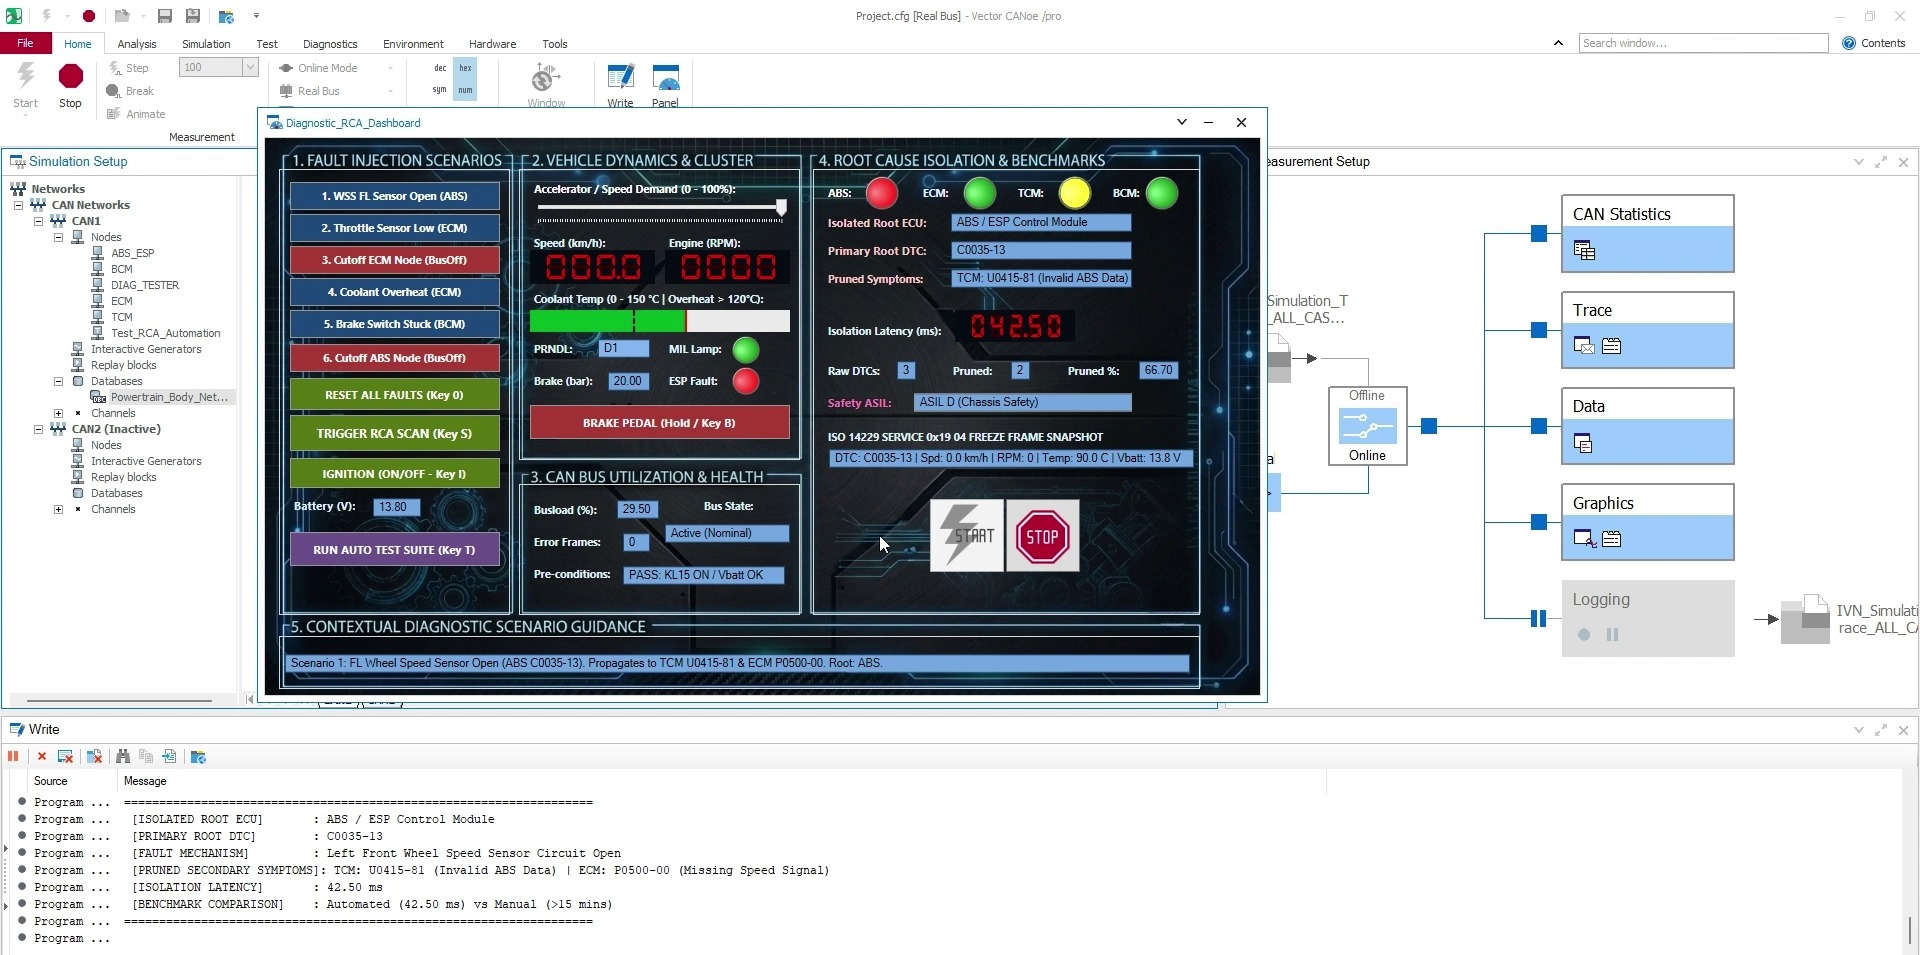
\includegraphics[width=0.98\linewidth, height=3.95cm, keepaspectratio]{video_poster.jpg}};
            \fill[vectorred, opacity=0.90] (vid.center) circle (0.48cm);
            \fill[white] ($(vid.center)+(-0.11,-0.19)$) -- ($(vid.center)+(0.23,0)$) -- ($(vid.center)+(-0.11,0.19)$) -- cycle;
          \end{tikzpicture}%
        }{../CB.EN.U4EEE23112_IVN_VIDEO.mp4}%
      }\\[5pt]
      \scriptsize\color{slatedark}
      \texttt{\textbf{CB.EN.U4EEE23112\_IVN\_VIDEO.mp4}}\\[2pt]
      1080p Full HD (30 fps) \quad\textbullet\quad 17 min 57 sec \quad\textbullet\quad 357.5 MB\\[2pt]
      {\color{vectorred}\textbf{Click video frame to launch playback}}
    \end{tcolorbox}
  \end{column}

  % Right Column: Video Breakdown Timeline Table
  \begin{column}{0.50\textwidth}
    \begin{tcolorbox}[whitecard, height=6.10cm]
      \textbf{\small\color{slatedark} Video Scenario Breakdown \& Cue Sheet}\\[5pt]
      \resizebox{\linewidth}{!}{%
      \scriptsize
      \setlength{\tabcolsep}{3pt}
      \renewcommand{\arraystretch}{1.42}
      \begin{tabular}{@{}lll@{}}
        \toprule
        \textbf{Timestamp} & \textbf{Phase} & \textbf{Key Observation / Proof Point} \\
        \midrule
        \textbf{00:00--02:45} & Baseline        & Nominal driving, zero DTCs \\
        \textbf{02:45--05:30} & Sc. 1 (WSS)     & Speed drops, ABS C0035-13 isolated \\
        \textbf{05:30--08:15} & Sc. 2 (APP)     & Throttle 0\%, ECM P0122-12 isolated \\
        \textbf{08:15--11:00} & Sc. 3 (Coolant) & 125$^\circ$C limit, ECM P0217-00 isolated \\
        \textbf{11:00--13:45} & Sc. 4 \& 6      & Node cutoffs: U0121 / U0100 isolated \\
        \textbf{13:45--17:57} & Sc. 5 (Brake)   & BTO coastdown, BCM B1318-11 isolated \\
        \bottomrule
      \end{tabular}%
      }\\[8pt]
      \footnotesize\color{slategrey}\raggedright
      Each recorded test proves periodic UDS Service 0x19 02 interrogation, real-time DAG pruning, and downstream DTC suppression in Vector CANoe 19.
    \end{tcolorbox}
  \end{column}

\end{columns}

\end{frame}

% =============================================================================
% SLIDE 9: Quantitative Results & State-of-the-Art Benchmark
% =============================================================================
\begin{frame}[t]
\slidetitle{Experimental Results \& State-of-the-Art Benchmark}{100\% Isolation Accuracy \textbullet{} 63.9\% DTC Suppression \textbullet{} 42.50 ms Interrogation Latency}

\begin{columns}[T,totalwidth=\textwidth]

  \begin{column}{0.485\textwidth}
    \begin{tcolorbox}[whitecard, colframe=vectorred!70, colbacktitle=vectorred!8, height=4.35cm,
      title={\footnotesize\bfseries\color{vectorred} Table I: Scenario Performance (6 Failure Modes)}]
      \centering
      \resizebox{\linewidth}{!}{%
      \scriptsize
      \setlength{\tabcolsep}{3pt}
      \renewcommand{\arraystretch}{1.24}
      \begin{tabular}{@{}lcccc@{}}
        \toprule
        \textbf{Scenario} & \textbf{ASIL} & \textbf{Raw} & \textbf{Suppressed} & \textbf{Latency} \\
        \midrule
        1: WSS Open Circuit    & D & 3 & 2 (66.7\%) & 42.10 ms \\
        2: Throttle Sensor Low & D & 2 & 1 (50.0\%) & 41.80 ms \\
        3: Coolant Overheat    & B & 3 & 2 (66.7\%) & 40.50 ms \\
        4: ABS Node Cutoff     & D & 3 & 2 (66.7\%) & 45.20 ms \\
        5: Brake Switch Stuck  & B & 3 & 2 (66.7\%) & 42.40 ms \\
        6: ECM Node Cutoff     & D & 3 & 2 (66.7\%) & 43.00 ms \\
        \midrule
        \textbf{Avg / Total} & \textbf{B--D} & \textbf{2.8 (17)} & \textbf{1.8 (63.9\%)} & \textbf{42.50 ms} \\
        \bottomrule
      \end{tabular}%
      }
    \end{tcolorbox}
  \end{column}

  \begin{column}{0.485\textwidth}
    \begin{tcolorbox}[whitecard, colframe=accentblue!70, colbacktitle=accentblue!8, height=4.35cm,
      title={\footnotesize\bfseries\color{accentblue} Table II: State-of-the-Art Comparative Benchmark}]
      \centering
      \resizebox{\linewidth}{!}{%
      \scriptsize
      \setlength{\tabcolsep}{2.6pt}
      \renewcommand{\arraystretch}{1.24}
      \begin{tabular}{@{}llccc@{}}
        \toprule
        \textbf{Framework} & \textbf{Method} & \textbf{Order} & \textbf{Latency} & \textbf{RAM} \\
        \midrule
        Lin \emph{et al.} (2023)  & Matrix Rules   & $O(N^2)$       & 120 ms  & 12.4 KB \\
        Liu \emph{et al.} (2023)  & Bayesian DAG   & $O(2^k |V|)$   & 340 ms  & 45.2 KB \\
        Wang \emph{et al.} (2023) & Wire Topo      & $O(N)$         & 210 ms  & 8.6 KB  \\
        Lu \emph{et al.} (2025)   & CNN-LSTM       & High           & 85 ms   & 5.8 MB  \\
        Bohne \emph{et al.} (2023)& Neuro-Sym      & NP-Hard        & 1250 ms & 22.1 MB \\
        \midrule
        \textbf{This Work}        & \textbf{DAG}   & $\mathbf{O(|V|{+}|E|)}$ & \textbf{42.5 ms} & $\mathbf{<320}$ \textbf{B} \\
        \bottomrule
      \end{tabular}%
      }
    \end{tcolorbox}
  \end{column}

\end{columns}

\vspace{0.20cm}
\begin{columns}[T,totalwidth=\textwidth]
  \begin{column}{0.235\textwidth}
    \begin{tcolorbox}[cardstyle, colframe=accentgreen!70, left=4pt, right=4pt, top=5pt, bottom=5pt, height=1.45cm]
      \centering{\large\bfseries\color{accentgreen} 100\%}\\[2pt]\scriptsize\color{slatedark}\textbf{Root Cause Accuracy}\\(6 / 6 Scenarios)
    \end{tcolorbox}
  \end{column}
  \begin{column}{0.235\textwidth}
    \begin{tcolorbox}[cardstyle, colframe=vectorred!70, left=4pt, right=4pt, top=5pt, bottom=5pt, height=1.45cm]
      \centering{\large\bfseries\color{vectorred} 63.9\%}\\[2pt]\scriptsize\color{slatedark}\textbf{DTC Flood Reduction}\\(11 of 17 Pruned)
    \end{tcolorbox}
  \end{column}
  \begin{column}{0.235\textwidth}
    \begin{tcolorbox}[cardstyle, colframe=accentblue!70, left=4pt, right=4pt, top=5pt, bottom=5pt, height=1.45cm]
      \centering{\large\bfseries\color{accentblue} 42.50 ms}\\[2pt]\scriptsize\color{slatedark}\textbf{Avg Isolation Latency}\\(ISO 26262 FTTI $<100$ ms)
    \end{tcolorbox}
  \end{column}
  \begin{column}{0.235\textwidth}
    \begin{tcolorbox}[cardstyle, colframe=nodetester!70, left=4pt, right=4pt, top=5pt, bottom=5pt, height=1.45cm]
      \centering{\large\bfseries\color{nodetester} $<8~\mu$s}\\[2pt]\scriptsize\color{slatedark}\textbf{AURIX TC397 Exec}\\(1840 cyc \textbar{} 320 B mem)
    \end{tcolorbox}
  \end{column}
\end{columns}

\end{frame}

% =============================================================================
% SLIDE 10: Key Learnings, Zonal Scalability & Conclusion
% =============================================================================
\begin{frame}[t]
\slidetitle{Key Learnings, Scalability \& Conclusion}{Industrial Takeaways \textbullet{} Zonal E/E Migration \textbullet{} Evaluator Q\&A Transition}

\begin{columns}[T,totalwidth=\textwidth]

  \begin{column}{0.485\textwidth}
    \begin{tcolorbox}[cardstyle, colframe=vectorred!70, colbacktitle=vectorred!8, height=5.20cm,
      title={\normalsize\bfseries\color{vectorred} Key Engineering Learnings}]
      \footnotesize\color{slatedark}\raggedright
      \begin{itemize}\setlength{\itemsep}{3.5pt}\setlength{\leftmargini}{10pt}
        \item \textbf{Causal Over Rule-Based:} In-degree topological pruning eliminates cascading symptom DTCs without maintaining brittle static rule tables.
        \item \textbf{Functional Safety Guarantee:} Cross-checking mechanical sensors (0.8 bar hydraulic pressure) against electrical contacts plus BTO prevents phantom braking and overspeed.
        \item \textbf{Embedded Determinism:} Linear $O(|V| + |E|)$ complexity runs in $<8~\mu$s on automotive silicon with 100\% deterministic fail-safe behavior under ISO 26262.
      \end{itemize}
    \end{tcolorbox}
  \end{column}

  \begin{column}{0.485\textwidth}
    \begin{tcolorbox}[cardstyle, colframe=accentblue!70, colbacktitle=accentblue!8, height=5.20cm,
      title={\normalsize\bfseries\color{accentblue} Zonal Scalability \& Future Roadmap}]
      \footnotesize\color{slatedark}\raggedright
      \begin{itemize}\setlength{\itemsep}{3.5pt}\setlength{\leftmargini}{10pt}
        \item \textbf{Zonal E/E Readiness:} Adjacency bitmasks map directly onto high-speed zonal gateways and central compute clusters with $<320$ bytes memory for 50 nodes.
        \item \textbf{Future Extensions:} Dynamic DAG generation from vendor DBC/ARXML databases, ISO 13400 DoIP over gigabit Automotive Ethernet, and CAN-XL physical transceivers.
      \end{itemize}
    \end{tcolorbox}
  \end{column}

\end{columns}

\vspace{0.15cm}
\begin{tcolorbox}[colback=accentgreen!12, colframe=accentgreen!60, boxrule=0.9pt, arc=5pt, left=10pt, right=10pt, top=7pt, bottom=7pt]
  \centering\normalsize\bfseries\color{accentgreen!90!black}
  THANK YOU! \quad\textbullet\quad OPEN FOR EVALUATOR QUESTIONS \& DISCUSSION
\end{tcolorbox}

\end{frame}

\end{document}
